\documentclass[
    11pt,
    aspectratio=169,
]{beamer}
\mode<beamer>{
\usetheme[hideothersubsections,
right,width=22mm]{Goettingen}
}
\usepackage[spanish]{babel} %Definir idioma español
\usepackage[utf8]{inputenc} %Codificacion utf-8
\usepackage{hyperref}
\title{Control continuo con aprendizaje por refuerzo profundo}
\author{Emmanuel Peto Gutiérrez}
\institute{IIMAS \\ UNAM}
\begin{document}

\begin{frame}<handout:0>
\titlepage
\end{frame}

\section{Aprendizaje por refuerzo}

% Frame
\begin{frame}
\frametitle{La interfaz agente-ambiente}

\begin{center}
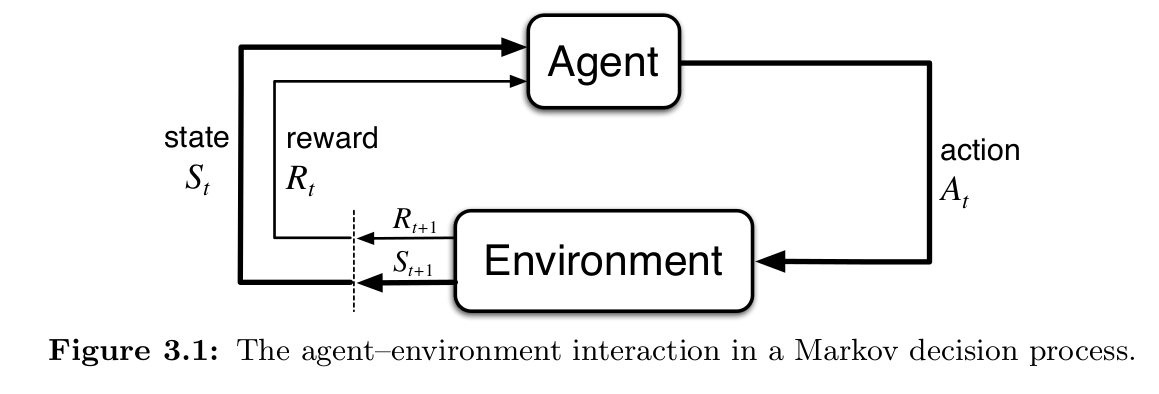
\includegraphics[scale=0.26]{Images/env_agent}
\end{center}

\end{frame}

% Frame
\begin{frame}
\frametitle{Actor-critic}

Un método actor-crítico aprende las funciones de aproximación tanto para la política como para la función de valor.

\begin{itemize}
\item Actor: la función relacionada con la política ($\pi (a|s)$ o $\mu (s)$).
\item Crítico: la función relacionada con el valor ($q(s,a)$ o $v(s)$).
\end{itemize}

\begin{center}
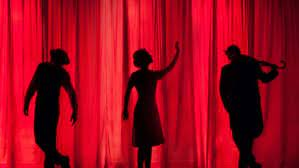
\includegraphics[scale=0.4]{Images/actores}
\end{center}

\end{frame}

% Frame
\begin{frame}
\frametitle{El problema}

\textbf{Problema:} encontrar una política donde las variables acción ($a$) y (estado) $s$ son continuas, y probar resultados en problemas de control físico (como balancear un péndulo o manejar un carro).

\begin{center}
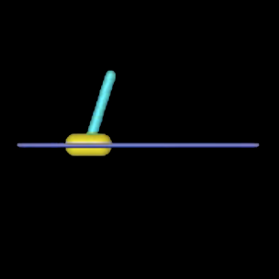
\includegraphics[scale=0.4]{Images/cartpole}
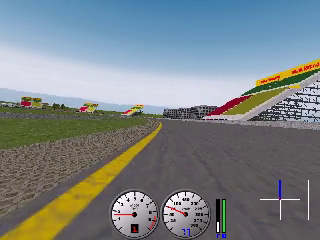
\includegraphics[scale=0.4]{Images/car_driving}
\end{center}

\end{frame}

\section{Agente y ambiente}

% Frame
\begin{frame}
\frametitle{Los agentes}

Para el agente se utilizaron los siguientes algoritmos:

\begin{itemize}
\item Deep Q-Network (DQN)
\item Deep Deterministic Policy Gradient (DDPG)
\end{itemize}

\end{frame}

% Frame
\begin{frame}
\frametitle{El ambiente}
Ambos algoritmos se probaron en el problema de cartpole, el cual consiste en balancear un péndulo moviendo el carro de manera horizontal.

\begin{center}
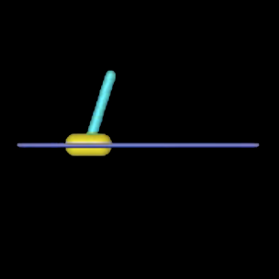
\includegraphics[scale=0.4]{Images/cartpole}
\end{center}

\end{frame}

% Frame
\begin{frame}
\frametitle{DQN vs DDPG}

\textbf{DQN}
\begin{itemize}
\item Aproxima directamente la función $Q$
\item Opera con acciones discretas
\item Solo tiene una red que aproxima $Q$
\end{itemize}

\textbf{DDPG}
\begin{itemize}
\item Aproxima una política determinista que maximice la esperanza
\item Opera con acciones continuas
\item Tiene dos redes, la que aproxima $Q$ y la que aproxima $\mu$
\end{itemize}

\end{frame}

\section{Resultados}

% Frame
\begin{frame}
\frametitle{Recompensa en DDPG}

Número de pasos: 40,000

\begin{center}
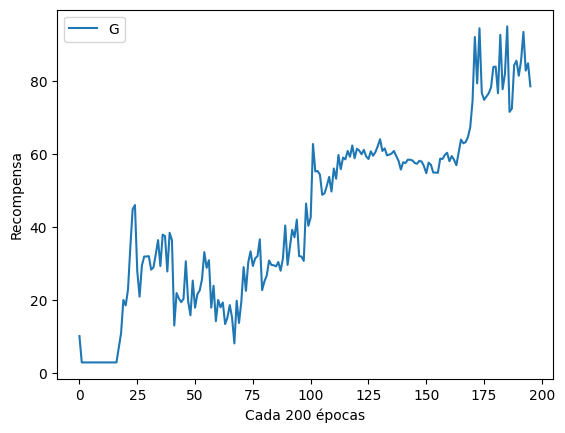
\includegraphics[scale=0.5]{Images/reward_ddpg}
\end{center}

\end{frame}

% Frame
\begin{frame}
\frametitle{Recompensa en DQN}

Número de episodios: 30,000

\begin{center}
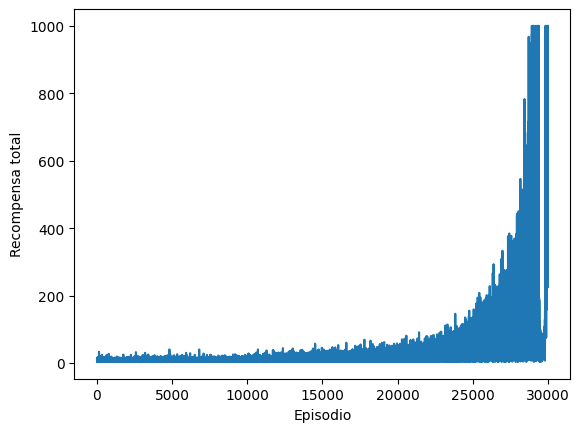
\includegraphics[scale=0.5]{Images/reward_dqn}
\end{center}

\end{frame}

\section{Conclusiones}

%Frame
\begin{frame}
\frametitle{Conclusiones}

\begin{itemize}
\item La discretización de las acciones para usar DQN puede resultar mejor que DDPG si la dimensión de la acción es baja.
\item El tiempo de cómputo de DQN puede ser mayor debido a que tiene que iterar sobre el espacio de estados discretizados.
\item El agente DDPG puede no apreder correctamente si el ruido es muy alto.
\end{itemize}

\end{frame}

\section{Apéndices}

\end{document}

